\documentclass[../main/main.tex]{subfiles}

\begin{document}
\espacio

  %------------ TODO ------------%
  En este capítulo se muestra el marco teórico TODO.

  \section{Antecedentes}

  \subsection{Computación paralela}

  La computación paralela es una rama de la informática que se encarga del estudio de la ejecución de una tarea dividida en sub-procesos o varias tareas independientes de forma simultánea en forma de hilos de ejecución en un grupo de procesadores llamados también procesadores multinúcleo, que luego de realizar dichas tareas sincronizan sus resultados a fin de mantener la integridad de los datos.

  \begin{figure}[H]
    \centering
    \caption{Disposición de un microprocesadores multinúcleo}
    \tikzset{every picture/.style={line width=0.75pt}} %set default line width to 0.75pt        

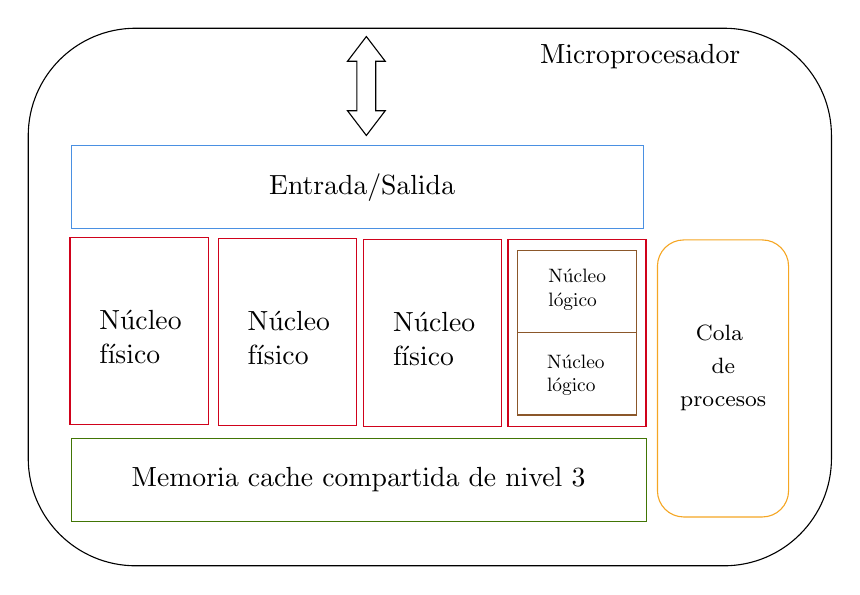
\begin{tikzpicture}[x=0.75pt,y=0.75pt,yscale=-1,xscale=1]
%uncomment if require: \path (0,300); %set diagram left start at 0, and has height of 300

%Shape: Rectangle [id:dp7451660985771589] 
\draw  [color={rgb, 255:red, 208; green, 2; blue, 27 }  ,draw opacity=1 ] (100.31,108) -- (166.81,108) -- (166.81,198.2) -- (100.31,198.2) -- cycle ;

%Shape: Rectangle [id:dp20887119442499946] 
\draw  [color={rgb, 255:red, 208; green, 2; blue, 27 }  ,draw opacity=1 ] (171.81,108.5) -- (238.31,108.5) -- (238.31,198.7) -- (171.81,198.7) -- cycle ;

%Shape: Rectangle [id:dp7286280016278224] 
\draw  [color={rgb, 255:red, 208; green, 2; blue, 27 }  ,draw opacity=1 ] (241.81,109) -- (308.31,109) -- (308.31,199.2) -- (241.81,199.2) -- cycle ;

%Shape: Rectangle [id:dp10536868660856769] 
\draw  [color={rgb, 255:red, 208; green, 2; blue, 27 }  ,draw opacity=1 ] (311.31,109) -- (377.81,109) -- (377.81,199.2) -- (311.31,199.2) -- cycle ;
%Shape: Rectangle [id:dp1826752439641639] 
\draw  [color={rgb, 255:red, 65; green, 117; blue, 5 }  ,draw opacity=1 ] (101.17,205.17) -- (378.06,205.17) -- (378.06,245.17) -- (101.17,245.17) -- cycle ;
%Rounded Rect [id:dp2234320479476144] 
\draw  [color={rgb, 255:red, 245; green, 166; blue, 35 }  ,draw opacity=1 ] (383.33,121.97) .. controls (383.33,114.99) and (388.99,109.33) .. (395.97,109.33) -- (433.87,109.33) .. controls (440.84,109.33) and (446.5,114.99) .. (446.5,121.97) -- (446.5,230.17) .. controls (446.5,237.14) and (440.84,242.8) .. (433.87,242.8) -- (395.97,242.8) .. controls (388.99,242.8) and (383.33,237.14) .. (383.33,230.17) -- cycle ;
%Shape: Rectangle [id:dp1417047542970684] 
\draw  [color={rgb, 255:red, 74; green, 144; blue, 226 }  ,draw opacity=1 ] (101,64) -- (376.5,64) -- (376.5,104) -- (101,104) -- cycle ;
%Shape: Rectangle [id:dp36104680527645483] 
\draw  [color={rgb, 255:red, 139; green, 87; blue, 42 }  ,draw opacity=1 ] (316,114.5) -- (373.25,114.5) -- (373.25,154.1) -- (316,154.1) -- cycle ;
%Shape: Rectangle [id:dp8737201655413631] 
\draw  [color={rgb, 255:red, 139; green, 87; blue, 42 }  ,draw opacity=1 ] (316,154.1) -- (373.25,154.1) -- (373.25,193.7) -- (316,193.7) -- cycle ;
%Rounded Rect [id:dp23562455979240182] 
\draw   (80.17,59.13) .. controls (80.17,30.52) and (103.36,7.33) .. (131.97,7.33) -- (415.37,7.33) .. controls (443.98,7.33) and (467.17,30.52) .. (467.17,59.13) -- (467.17,214.53) .. controls (467.17,243.14) and (443.98,266.33) .. (415.37,266.33) -- (131.97,266.33) .. controls (103.36,266.33) and (80.17,243.14) .. (80.17,214.53) -- cycle ;
%Up Down Arrow [id:dp8508564601094952] 
\draw   (234,23.25) -- (243.08,11.33) -- (252.17,23.25) -- (247.62,23.25) -- (247.62,47.08) -- (252.17,47.08) -- (243.08,59) -- (234,47.08) -- (238.54,47.08) -- (238.54,23.25) -- cycle ;

% Text Node
\draw (134.25,156) node  [align=left] {Núcleo\\ físico};
% Text Node
\draw (205.75,156.5) node  [align=left] {Núcleo\\ físico};
% Text Node
\draw (275.75,157) node  [align=left] {Núcleo\\ físico};
% Text Node
\draw (239.33,224.67) node  [align=left] {Memoria cache compartida de nivel 3};
% Text Node
\draw (415,171) node  [align=left] {{\footnotesize  \ \ Cola}\\{\footnotesize  \ \ \ \ de}\\{\footnotesize procesos}};
% Text Node
\draw (241,84) node  [align=left] {Entrada/Salida};
% Text Node
\draw (344.67,133.33) node [scale=0.7] [align=left] {Núcleo\\ lógico};
% Text Node
\draw (344,174.33) node [scale=0.7] [align=left] {Núcleo\\ lógico};
% Text Node
\draw (375,21) node  [align=left] {Microprocesador};


\end{tikzpicture}
    \caption*{\textbf{Fuente:} Elaboración propia}
  \end{figure}

  Los microprocesadores actuales contienen comúnmente dos tipos de núcleos, los núcleos físicos y los núcleos lógicos. Cada zócalo de una tarjeta madre contiene un microprocesador, este contiene uno o más núcleos físicos; un núcleo físico es aquel que se encuentra físicamente dentro del circuito integrado del microprocesador, mientras que un núcleo lógico es una división virtual en 2 o más partes de un núcleo físico. Las tareas son asignadas a los núcleos físicos; estas tareas pueden dividirse en tareas más pequeñas a fin de resolver un gran problema en partes pequeñas que al final serán unidas para generar la solución, estas partes pequeñas son llamadas ``hilos'' y son las que se ejecutan en los núcleo lógicos.

  \textit{Las técnicas principales para lograr estas mejoras de rendimiento (mayor frecuencia de reloj y arquitecturas cada vez más inteligentes y complejas) están golpeando la llamada ``Power Wall''. La industria informática ha aceptado que los futuros aumentos en rendimiento deben provenir en gran parte del incremento del número de procesadores (o núcleos) en una matriz, en vez de hacer más rápido un solo núcleo.} [\cite[p.~6]{report:parallel_computing_illinois}]

  El incremento de la frecuencia en los microprocesador acarrea consigo el consumo de energía y la disminución del espacio entre los transistores dentro de cada núcleo, lo que provoca un incremento considerable de la temperatura dentro del microprocesador; por tanto, para mantener el microprocesador en funcionamiento evitando su deterioro por las temperaturas elevadas es necesario buscar fuentes más óptimas de enfriado como los tubos de conducción de gas o líquido, que incrementan aún más el consumo de energía y que son costosos para una PC de escritorio.

  \begin{equation}
    T_m = T_a \cdot [( 1 - F_m ) + \frac{F_m}{A_m}]
    \label{ecuacion_amdahl}
  \end{equation}

  Donde:

  \begin{description}[noitemsep, nolistsep]
    \item[$F_m=$] Fracción de tiempo que el sistema utiliza el subsistema mejorado
    \item[$A_m=$] Factor de mejora que se ha introducido en el subsistema mejorado
    \item[$T_a=$] Tiempo de ejecución antiguo
    \item[$T_m=$] Tiempo de ejecución mejorado
  \end{description}

  Por tales motivos Gene Amdahl formuló la ecuación \ref{ecuacion_amdahl} que establece que:

  \textit{La mejora obtenida en el rendimiento de un sistema debido a la alteración de uno de sus componentes está limitada por la fracción de tiempo que se utiliza dicho componente}

  Despejando la ecuación \ref{ecuacion_amdahl} se obtiene la aceleración del programa completo una vez que se haya paralelizado uno o más algoritmos del programa.

  \begin{equation}
    A = \frac{1}{( 1 - F_m ) + \frac{F_m}{A_m}}
    \label{ecuacion_amdahl_aceleracion}
  \end{equation}

  Donde:

  \begin{description}[noitemsep, nolistsep]
    \item[$A=$] Aceleración o ganancia en velocidad conseguida en el sistema completo debido a la mejora de uno de sus subsistemas
    \item[$A_m=$] Factor de mejora que se ha introducido en el subsistema mejorado
    \item[$F_m=$] Fracción de tiempo que el sistema utiliza el subsistema mejorado
  \end{description}

  \begin{figure}[H]
    \centering
    \caption{Clúster de alto rendimiento}
    \includegraphics[width=10cm, keepaspectratio]{marco_teorico/cluster_alto_rendimiento.jpg}
    \caption*{\textbf{Fuente:} \cite[p.~2]{article:cluster_alto_rendimiento}}
  \end{figure}

  En base a este principio se desarrollaron tecnologías de matrices de núcleos de cómputo tomando como elementos principales a los procesadores existentes y acomodándolos de tal forma que se pueda administrar la ejecución de tareas en cada procesador de manera individual y la sincronización de resultados al final del proceso. Estos arreglos reciben el nombre de clústers. Los clústers de alto rendimiento son un tipo de clústers utilizados con el propósito de ejecutar tareas exhaustivas divididas en tareas pequeñas ejecutadas en cada computador de acuerdo a la gestión realizada por el llamado nodo maestro. [\cite{article:cluster_alto_rendimiento}]

  \begin{figure}[H]
    \centering
    \caption{Comparación de tiempos de proceso en múltiples CPUs}
    \includegraphics[width=15cm, keepaspectratio]{marco_teorico/resultado_cpu_cluster.png}
    \caption*{\textbf{Fuente:} \cite[p.~7]{article:cluster_alto_rendimiento}}
  \end{figure}

  \subsection{Unidad de procesamiento gráfico (GPU)}

  Esta unidad actúa como un co-procesador que se encarga de las operaciones matriciales o de coma flotante, por lo general los procesos gráficos de transformación o renderización son distribuidos a la o las GPUs desde el procesador central o CPU.

  Dado el estudio generado sobre las plataformas GPU, los fabricantes pusieron a disposición de los usuarios herramientas de desarrollo para utilizar las GPU como ayuda en cálculos de álgebra dispersa, tensores en dinámica de fluidos, minería de datos, inteligencia artificial, deep learning, etc, con lo cual la denominación de las GPU abiertas a otro tipo de uso más que el simple uso gráfico cambió a GPGPU\footnote{Unidad de Procesamiento Gráfico de Uso General (General Purpose Graphics Processing Unit)}.

  Estas tarjetas están desarrolladas en base al paralelismo de núcleos de frecuencia baja con un esquema de operaciones limitado.

  \begin{figure}[H]
    \centering
    \caption{Cantidad de núcleos en CPU vs GPU}
    \includegraphics[width=16cm, keepaspectratio]{marco_teorico/cpu_vs_gpu_cores.jpg}
    \caption*{\textbf{Fuente:} \cite{web:gpgpu}}
  \end{figure}

  El obstáculo principal para el desarrollo de aplicaciones orientadas hacia la GPU es que las arquitecturas de las tarjetas gráficas son demasiado variables, a pesar de la existencia de librerías o APIs genéricas como OpenGL, muchas funcionalidades dentro de los métodos o clases son variables entre fabricantes e incluso entre modelos de dispositivos de un mismo fabricante. Las librerías genéricas utilizan un núcleo basado en el esquema de Conductos de Renderización\footnote{Rendering Pipeline}, con los que se pueden tratar vectores, mapas de bits y elementos definidos pixel-pixel.

  Otro factor importante que impide hacer un uso adecuado de estos dispositivos es el límite físico con el que actualmente cuenta la conexión de memoria RAM de la GPU con el bus de la CPU para la transferencia de datos. Al cuarto trimestre de 2018 ya se cuenta con la tecnología GDDR6\footnote{Tasa Doble de transferencia de Datos  (Double Data Rate)} que ofrece un ancho de banda de hasta 16Gbps frente a los 10Gbps de su predecesor GDDR5X, cabe mencionar que se lograron estos anchos de banda gracias al cambio de modo half-duplex o transferencia en ambos sentidos pero solo uno a la vez, por el modo full-duplex que transfiere los datos en ambos sentidos al mismo tiempo.

  \begin{figure}[H]
    \centering
    \caption{Comparación de tecnologías GDDR6 vs GDDR5}
    \includegraphics[width=12cm, keepaspectratio]{marco_teorico/comparacion_gddr.png}
    \caption*{\textbf{Fuente:} \cite{web:comparacion_gddr}}
  \end{figure}

  Pero AMD ya se encuentra desarrollando tarjetas madres con conectores PCI-E\footnote{Componente Periférico de Interconexión Expresa (Peripheral Component Interconnect Express)} 5.0 que incrementarán la velocidad de transferencia hasta los 32Gbps que conjuntamente con el almacenamiento SSD\footnote{Solid State Drive} lograrán impulsar el desarrollo de aplicaciones de uso general en las GPUs.

  \begin{table}[H]
    \centering
    \caption{Comparación de tecnologías PCI-E}
    \begin{tabular}{c|c|c|c|c|}
  \cline{2-5}
                                          & \textbf{RAW Bitrate} & \textbf{Link BW} & \textbf{BW/Lane/Way} & \textbf{Total BW X16} \\ \hline
  \multicolumn{1}{|c|}{\textbf{PCIe 1.x}} & 2.5 GT/s             & 2 Gb/s           & 250 MB/s             & 8 GB/s                \\ \hline
  \multicolumn{1}{|c|}{\textbf{PCIe 2.x}} & 5.0 GT/s             & 4 Gb/s           & 500 MB/s             & 16 GB/s               \\ \hline
  \multicolumn{1}{|c|}{\textbf{PCIe 3.x}} & 8.0 GT/s             & 8 Gb/s           & $\sim$1 GB/s         & $\sim$32 GB/s         \\ \hline
  \multicolumn{1}{|c|}{\textbf{PCIe 4.x}} & 16 GT/s              & 16 Gb/s          & $\sim$2 GB/s         & $\sim$64 GB/s         \\ \hline
  \multicolumn{1}{|c|}{\textbf{PCIe 5.x}} & 32 GT/s              & 32 Gb/s          & $\sim$4 GB/s         & $\sim$128 GB/s        \\ \hline
  \end{tabular}
    \caption*{\textbf{Fuente:} \cite{web:comparacion_pcie}}
  \end{table}

  \section{AES}

  El Estándar de Encriptación Avanzada fue de desarrollado mediante un concurso en 1997, por los criptógrafos Vincent Rijmen e Joan Daemen en el año 2001, como la sustitución al algoritmo DES\footnote{Estándar de Encriptación de Datos(Data Encryption Standard)} que había sido crackeado mediante la máquina DES Cracker construida por la ONG Electronic Frontier Foundation, con una inversión de 250 mil dólares. Este estándar fue aprobado y es utilizado por entes reguladores como la NSA\footnote{Agencia de Seguridad Nacional(National Security Agency)} y se estandariza mediante la norma ISO/IEC 18033 [\cite{standard:iso_18033}].

  El algoritmo AES Rijndael es un algoritmo de llave simétrica, lo cual indica que se utiliza una misma llave para cifrar y descifrar los mensajes en el lado del emisor y del receptor. Por tal razón, toda la seguridad recae en proteger la clave secreta, por tal razón el abanico de claves posibles debe ser de una cantidad tan grande que el intruso deba realizar pruebas, por inclusive años, para poder descifrar el mensaje. Para el caso de DES, la clave es de 56 bits por lo que la cantidad de claves será igual a: $2^{56} = 7.2 \times 10^{16}$ posibles claves; un computador actual puede lograr descifrar un mensaje mediante el cálculo de la llave secreta en un tiempo de tan solo segundos.

  \begin{table}[H]
    \centering
    \caption{Comparación de tecnologías PCI-E}
    \begin{tabular}{|c|c|}
  \hline
  \multicolumn{1}{|l|}{\textbf{Tamaño de Clave}} & \multicolumn{1}{l|}{\textbf{Combinaciones Posibles}} \\ \hline
  1 bit & $2$ \\ \hline
  2 bit & $4$ \\ \hline
  4 bit & $16$ \\ \hline
  8 bit & $256$ \\ \hline
  16 bit & $65536$ \\ \hline
  32 bit & $4.2\times10^{9}$ \\ \hline
  56 bit (DES) & $7.2\times10^{16}$ \\ \hline
  64 bit & $1.8\times10^{19}$ \\ \hline
  128 bit (AES) & $3.4\times10^{38}$ \\ \hline
  192 bit (AES) & $6.2\times10^{57}$ \\ \hline
  256 bit (AES) & $1.1\times10^{77}$ \\ \hline
  \end{tabular}
    \caption*{\textbf{Fuente:} \cite{web:tiempo_crack_aes}}
  \end{table}

  El algoritmo AES Rijndael trabaja con mensajes divididos en bloques de 128 bits y llaves de logitud de 128, 192 y 256 bits. Por lo tanto con una llave de 128 bits el atacante necesitaría generar: $2^{56} = 3.4 \times 10^{38}$ llaves, tarea que en la actualidad, aún con computadoras tan potentes, el trabajo tardaría millones de años.

  Suponiendo la super-computadora Summit de IBM [\cite{web:supercomputadora_summit_ibm}], designada para descifrar un mensaje, trabajando a $143.5PFlops$\footnote{Operaciones de Punto Flotante por Segundo(Floating point Operations Per Second)} o $143.5 \times 10^{15} Flops$ y sabiendo que la cantidad de segundos en un año es de: $365 x 24 x 60 x 60 = 31536000$. Se calcula la cantidad de años necesarios para crackear AES con una longitud de clave de 128 bits.


  \begin{equation}
    \begin{aligned}
    t &= \frac{3.4 \times 10^{38}}{143.5 \times 10^{15} x 31536000} \\
    t &= \frac{23.69 \times 10^{15}}{315.36} \\
    t &= 75.13 \times 10^{12} a\tilde{n}os
    \end{aligned}
  \end{equation}

  Es decir, con la última tecnología disponible actualmente se tomaría un tiempo de 75.13 billones de años en generar las llaves secretas necesarias para descifrar un mensaje. Suponiendo que solo fuese necesario generar la mitad de las llaves para encontrar la correcta, el proceso tardaría mas de 32 billones de años. Por lo tanto una llave secreta de 128 bits utilizada para cifrar un mensaje con el algoritmo AES Rijndael es suficiente seguridad para la actualidad y para unos años más en el futuro.

  \subsection{Etapas del cifrado AES Rijndael}



  \begin{figure}[H]
    \centering
    \caption{Algoritmo AES Rijndael}
    \tikzset{every picture/.style={line width=0.75pt}} %set default line width to 0.75pt        

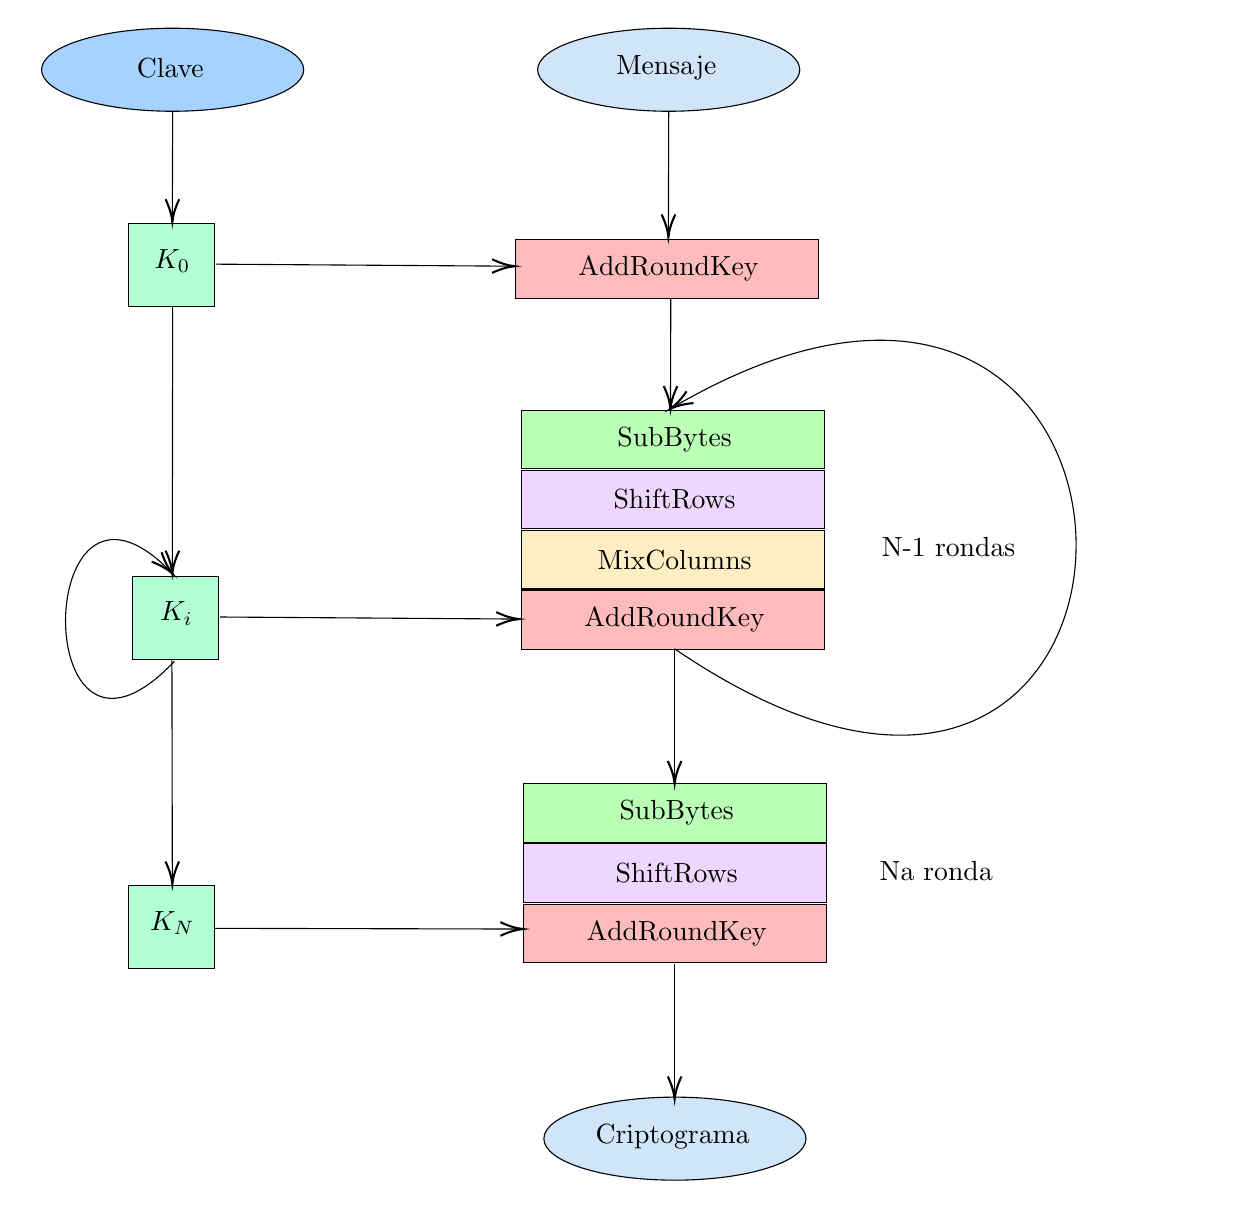
\begin{tikzpicture}[x=0.75pt,y=0.75pt,yscale=-1,xscale=1]
%uncomment if require: \path (0,607.4630661010742); %set diagram left start at 0, and has height of 607.4630661010742

%Shape: Ellipse [id:dp9737685907668199] 
\draw  [color={rgb, 255:red, 0; green, 0; blue, 0 }  ,draw opacity=1 ][fill={rgb, 255:red, 165; green, 210; blue, 255 }  ,fill opacity=1 ] (104,40) .. controls (104,28.95) and (132.27,20) .. (167.15,20) .. controls (202.03,20) and (230.3,28.95) .. (230.3,40) .. controls (230.3,51.05) and (202.03,60) .. (167.15,60) .. controls (132.27,60) and (104,51.05) .. (104,40) -- cycle ;

%Shape: Ellipse [id:dp45013119054902284] 
\draw  [color={rgb, 255:red, 0; green, 0; blue, 0 }  ,draw opacity=1 ][fill={rgb, 255:red, 208; green, 229; blue, 249 }  ,fill opacity=1 ] (343,40) .. controls (343,28.95) and (371.27,20) .. (406.15,20) .. controls (441.03,20) and (469.3,28.95) .. (469.3,40) .. controls (469.3,51.05) and (441.03,60) .. (406.15,60) .. controls (371.27,60) and (343,51.05) .. (343,40) -- cycle ;

%Shape: Rectangle [id:dp657856114899342] 
\draw  [fill={rgb, 255:red, 178; green, 255; blue, 211 }  ,fill opacity=1 ] (146,114) -- (187.3,114) -- (187.3,154) -- (146,154) -- cycle ;

%Shape: Rectangle [id:dp261406348143415] 
\draw  [fill={rgb, 255:red, 178; green, 255; blue, 211 }  ,fill opacity=1 ] (148,284) -- (189.3,284) -- (189.3,324) -- (148,324) -- cycle ;

%Shape: Rectangle [id:dp9188720632833878] 
\draw  [fill={rgb, 255:red, 178; green, 255; blue, 211 }  ,fill opacity=1 ] (146,433) -- (187.3,433) -- (187.3,473) -- (146,473) -- cycle ;

%Shape: Rectangle [id:dp25111749195065625] 
\draw  [fill={rgb, 255:red, 254; green, 187; blue, 187 }  ,fill opacity=1 ] (332.3,122) -- (478.3,122) -- (478.3,150.2) -- (332.3,150.2) -- cycle ;

%Shape: Rectangle [id:dp9024991354173098] 
\draw  [fill={rgb, 255:red, 187; green, 255; blue, 182 }  ,fill opacity=1 ] (335.3,204) -- (481.3,204) -- (481.3,232.2) -- (335.3,232.2) -- cycle ;

%Shape: Rectangle [id:dp6677044127286271] 
\draw  [fill={rgb, 255:red, 238; green, 214; blue, 255 }  ,fill opacity=1 ] (335.3,233) -- (481.3,233) -- (481.3,261.2) -- (335.3,261.2) -- cycle ;

%Shape: Rectangle [id:dp5668522361712407] 
\draw  [fill={rgb, 255:red, 255; green, 237; blue, 195 }  ,fill opacity=1 ] (335.3,262) -- (481.3,262) -- (481.3,290.2) -- (335.3,290.2) -- cycle ;

%Shape: Rectangle [id:dp34737624535273803] 
\draw  [fill={rgb, 255:red, 254; green, 187; blue, 187 }  ,fill opacity=1 ] (335.3,291) -- (481.3,291) -- (481.3,319.2) -- (335.3,319.2) -- cycle ;

%Shape: Rectangle [id:dp4367963290792771] 
\draw  [fill={rgb, 255:red, 187; green, 255; blue, 182 }  ,fill opacity=1 ] (336.3,384) -- (482.3,384) -- (482.3,412.2) -- (336.3,412.2) -- cycle ;

%Shape: Rectangle [id:dp012716397520244005] 
\draw  [fill={rgb, 255:red, 238; green, 214; blue, 255 }  ,fill opacity=1 ] (336.3,413) -- (482.3,413) -- (482.3,441.2) -- (336.3,441.2) -- cycle ;

%Shape: Rectangle [id:dp1945157717160817] 
\draw  [fill={rgb, 255:red, 254; green, 187; blue, 187 }  ,fill opacity=1 ] (336.3,442) -- (482.3,442) -- (482.3,470.2) -- (336.3,470.2) -- cycle ;

%Shape: Ellipse [id:dp0074509944076393] 
\draw  [color={rgb, 255:red, 0; green, 0; blue, 0 }  ,draw opacity=1 ][fill={rgb, 255:red, 208; green, 229; blue, 249 }  ,fill opacity=1 ] (346,555) .. controls (346,543.95) and (374.27,535) .. (409.15,535) .. controls (444.03,535) and (472.3,543.95) .. (472.3,555) .. controls (472.3,566.05) and (444.03,575) .. (409.15,575) .. controls (374.27,575) and (346,566.05) .. (346,555) -- cycle ;

%Straight Lines [id:da2019009163904124] 
\draw    (167.15,60) -- (167.01,111.33) ;
\draw [shift={(167,113.33)}, rotate = 270.15999999999997] [color={rgb, 255:red, 0; green, 0; blue, 0 }  ][line width=0.75]    (10.93,-3.29) .. controls (6.95,-1.4) and (3.31,-0.3) .. (0,0) .. controls (3.31,0.3) and (6.95,1.4) .. (10.93,3.29)   ;

%Straight Lines [id:da7298574790525367] 
\draw    (406.15,60) -- (406,118.67) ;
\draw [shift={(406,120.67)}, rotate = 270.14] [color={rgb, 255:red, 0; green, 0; blue, 0 }  ][line width=0.75]    (10.93,-3.29) .. controls (6.95,-1.4) and (3.31,-0.3) .. (0,0) .. controls (3.31,0.3) and (6.95,1.4) .. (10.93,3.29)   ;

%Straight Lines [id:da12255807726786161] 
\draw    (188,133.67) -- (330,134.65) ;
\draw [shift={(332,134.67)}, rotate = 180.4] [color={rgb, 255:red, 0; green, 0; blue, 0 }  ][line width=0.75]    (10.93,-3.29) .. controls (6.95,-1.4) and (3.31,-0.3) .. (0,0) .. controls (3.31,0.3) and (6.95,1.4) .. (10.93,3.29)   ;

%Straight Lines [id:da15131688097810092] 
\draw    (407.15,150) -- (407.01,201.33) ;
\draw [shift={(407,203.33)}, rotate = 270.15999999999997] [color={rgb, 255:red, 0; green, 0; blue, 0 }  ][line width=0.75]    (10.93,-3.29) .. controls (6.95,-1.4) and (3.31,-0.3) .. (0,0) .. controls (3.31,0.3) and (6.95,1.4) .. (10.93,3.29)   ;

%Straight Lines [id:da5876036775611393] 
\draw    (190,303.67) -- (332,304.65) ;
\draw [shift={(334,304.67)}, rotate = 180.4] [color={rgb, 255:red, 0; green, 0; blue, 0 }  ][line width=0.75]    (10.93,-3.29) .. controls (6.95,-1.4) and (3.31,-0.3) .. (0,0) .. controls (3.31,0.3) and (6.95,1.4) .. (10.93,3.29)   ;

%Straight Lines [id:da031674005498631086] 
\draw    (167.15,154) -- (167,280.67) ;
\draw [shift={(167,282.67)}, rotate = 270.07] [color={rgb, 255:red, 0; green, 0; blue, 0 }  ][line width=0.75]    (10.93,-3.29) .. controls (6.95,-1.4) and (3.31,-0.3) .. (0,0) .. controls (3.31,0.3) and (6.95,1.4) .. (10.93,3.29)   ;

%Curve Lines [id:da11017760368079688] 
\draw    (409,319) .. controls (666.24,494.29) and (668.24,49.29) .. (407,203.33) ;
\draw [shift={(407,203.33)}, rotate = 329.47] [color={rgb, 255:red, 0; green, 0; blue, 0 }  ][line width=0.75]    (10.93,-3.29) .. controls (6.95,-1.4) and (3.31,-0.3) .. (0,0) .. controls (3.31,0.3) and (6.95,1.4) .. (10.93,3.29)   ;

%Curve Lines [id:da7191324048148082] 
\draw    (168,325) .. controls (97.57,399.34) and (99.2,213.59) .. (165.99,281.62) ;
\draw [shift={(167,282.67)}, rotate = 226.31] [color={rgb, 255:red, 0; green, 0; blue, 0 }  ][line width=0.75]    (10.93,-3.29) .. controls (6.95,-1.4) and (3.31,-0.3) .. (0,0) .. controls (3.31,0.3) and (6.95,1.4) .. (10.93,3.29)   ;

%Straight Lines [id:da034441479180648216] 
\draw    (166.8,324.33) -- (167,430.4) ;
\draw [shift={(167,432.4)}, rotate = 269.89] [color={rgb, 255:red, 0; green, 0; blue, 0 }  ][line width=0.75]    (10.93,-3.29) .. controls (6.95,-1.4) and (3.31,-0.3) .. (0,0) .. controls (3.31,0.3) and (6.95,1.4) .. (10.93,3.29)   ;

%Straight Lines [id:da40164122139794234] 
\draw    (409,319) -- (409,382) ;
\draw [shift={(409,384)}, rotate = 270] [color={rgb, 255:red, 0; green, 0; blue, 0 }  ][line width=0.75]    (10.93,-3.29) .. controls (6.95,-1.4) and (3.31,-0.3) .. (0,0) .. controls (3.31,0.3) and (6.95,1.4) .. (10.93,3.29)   ;

%Straight Lines [id:da19063932307712084] 
\draw    (187,453.67) -- (334,454) ;
\draw [shift={(336,454)}, rotate = 180.13] [color={rgb, 255:red, 0; green, 0; blue, 0 }  ][line width=0.75]    (10.93,-3.29) .. controls (6.95,-1.4) and (3.31,-0.3) .. (0,0) .. controls (3.31,0.3) and (6.95,1.4) .. (10.93,3.29)   ;

%Straight Lines [id:da027755398290204125] 
\draw    (409,471) -- (409,534) ;
\draw [shift={(409,536)}, rotate = 270] [color={rgb, 255:red, 0; green, 0; blue, 0 }  ][line width=0.75]    (10.93,-3.29) .. controls (6.95,-1.4) and (3.31,-0.3) .. (0,0) .. controls (3.31,0.3) and (6.95,1.4) .. (10.93,3.29)   ;


% Text Node
\draw (166,39) node  [align=left] {Clave};
% Text Node
\draw (405,39) node  [align=left] {Mensaje};
% Text Node
\draw (167,132) node   {$K_{0}$};
% Text Node
\draw (169,302) node   {$K_{i}$};
% Text Node
\draw (167,451) node   {$K_{N}$};
% Text Node
\draw (406,136) node  [align=left] {AddRoundKey};
% Text Node
\draw (409,218) node  [align=left] {SubBytes};
% Text Node
\draw (409,247) node  [align=left] {ShiftRows};
% Text Node
\draw (409,276) node  [align=left] {MixColumns};
% Text Node
\draw (409,305) node  [align=left] {AddRoundKey};
% Text Node
\draw (410,456) node  [align=left] {AddRoundKey};
% Text Node
\draw (410,427) node  [align=left] {ShiftRows};
% Text Node
\draw (410,398) node  [align=left] {SubBytes};
% Text Node
\draw (408,554) node  [align=left] {Criptograma};
% Text Node
\draw (541,270) node  [align=left] {N-1 rondas};
% Text Node
\draw (535,426) node  [align=left] {Na ronda};


\end{tikzpicture}

    \caption*{\textbf{Fuente:} Elaboración propia}
  \end{figure}


\end{document}